\subsection{Operational policy requirements and outcome associations}
The policy corpus assigns distinct, overlapping responsibilities to operation after construction. Among \PolicyDocs{} locally applicable policy documents covering \PolicyCities{} cities, \RequirementDocs{} documents covering \RequirementCities{} cities provide \RequirementClauses{} clauses for the analysis of operational requirements. Information and supervision appear in \InformationCities{} cities, compared with \MaintenanceCities{} for operation and maintenance, \ContinuityCities{} for continuing-operation or payment conditions, and \AssessableCities{} for assessable or subsidy-linked requirements. These counts describe what documents prescribe, not implementation; a clause can carry more than one functional label.

The content counts use an 88-city requirement scope, whereas the administrative sequence uses a separate 95-city governance registry. The scopes are therefore complementary rather than a single panel sample. The clauses identify concrete objects of responsibility: Suzhou requires real-time safety monitoring, Wuhan addresses compatibility across operator information and payment systems, Haikou specifies holiday-service provisions, and Shaoxing addresses resource use and charging spaces occupied by non-charging vehicles \citep{gov12,gov5,gov7,gov11}. Dongguan links platform connection and stable operation for at least five years to eligibility, while a separate settlement rule makes remaining subsidy payable after one year of normal operation \citep{gov1}. These provisions distinguish information, equipment condition, access and continuity from a generic facility count. Their functional coverage and administrative sequence are summarized in Figure~\ref{fig:policy}, with clause definitions and source locators in SI Section~\siref{sec:si-policy}.

The administrative timing also varies. In the \GovernanceCities-city registry, \BFirstCount{} cities have an earlier construction-support effective year and \SameYearCount{} share the year. The first-document division is \SameDocumentCities{} cities sharing the first document, \DifferentDocumentCities{} with different first documents and one unresolved case. All first governance documents contain construction support, so the observed sequence includes both joint introduction and governance following earlier support. It does not support a universal progression in which construction is always followed by a later operational correction.

The annual association uses the same 325 city-years under both specifications (Table~\ref{tab:policy_associations}). Prior-year-end information/supervision exposure is positively associated with log activity in the index-adjusted specification: \PolicyRActivity\ [\PolicyRActivityLow, \PolicyRActivityHigh]. Its facility and intensity intervals include zero, with the intensity coefficient \PolicyRIntensity\ [\PolicyRIntensityLow, \PolicyRIntensityHigh]. All operation/maintenance confidence intervals include zero; their widths vary across outcomes. Adding the pandemic-response index changes the common-sample estimates little. The models include city and year effects, four annual weather measures and province-clustered inference. The complete policy matrix and all weather-adjustment terms are reported in SI Section~\siref{sec:si-associations}. Because information obligations may alter reporting visibility as well as service, the positive activity association does not identify a single channel.

The governance extension covers 11 cities and 36 post-policy quarters against a comparison pool of 70 cities and 702 quarters. Its activity-minus-facility contrast is \HOneD. Facility leads differ systematically from the comparison benchmark, with joint $p=\PreNP$, so the contrast does not support a causal interpretation based on comparable untreated trajectories. The full target/comparison definitions, lead diagnostic and window decomposition are in SI Section~\siref{sec:si-governance}; SI Section~\siref{sec:si-trajectories} aligns the 11 target cities' activity, facilities and observation coverage. The documented functions, annual associations and quarterly extension therefore provide complementary evidence: they specify responsibilities, describe conditional correlations and expose a timing diagnostic, but do not form an identified policy-to-activity mediation chain.
\begin{table}[htbp]\centering\small\caption{Policy functions and charging outcomes}\label{tab:policy_associations}
\begin{tabular}{@{}p{43mm}lrr@{}}\toprule
\multicolumn{4}{l}{Same 325 city--years, 94 cities and 25 province clusters in both specifications}\\\midrule
Policy term & Outcome & \shortstack{Without COVID index\\Coefficient [95\% CI]} & \shortstack{With COVID index\\Coefficient [95\% CI]}\\
\midrule
Information/supervision $R$ & $\ln A$ & 1.770 [0.413, 3.127] & 1.739 [0.383, 3.096]\\
Information/supervision $R$ & $\ln N$ & 0.663 [-0.199, 1.524] & 0.661 [-0.210, 1.532]\\
Information/supervision $R$ & $\ln I$ & 1.107 [-0.236, 2.451] & 1.079 [-0.268, 2.425]\\
Operation/maintenance $S$ & $\ln A$ & -0.027 [-1.542, 1.489] & -0.034 [-1.562, 1.495]\\
Operation/maintenance $S$ & $\ln N$ & 0.418 [-0.696, 1.531] & 0.417 [-0.702, 1.537]\\
Operation/maintenance $S$ & $\ln I$ & -0.445 [-1.503, 0.614] & -0.451 [-1.522, 0.620]\\
\bottomrule\end{tabular}\end{table}

\begin{figure}[htbp]\centering
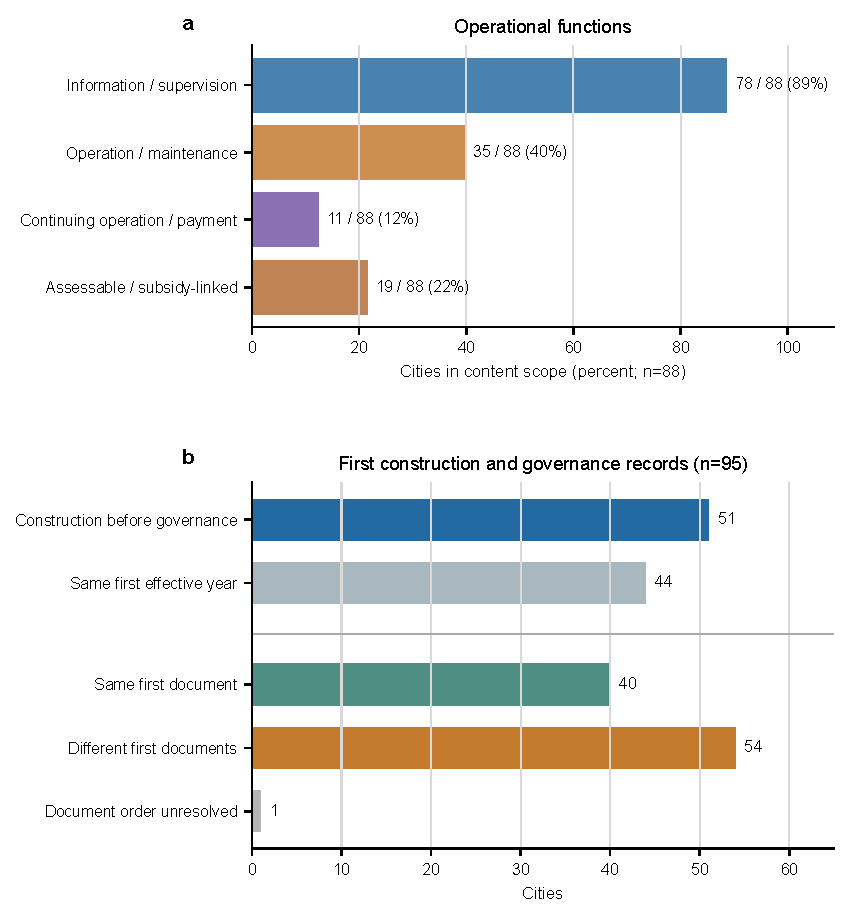
\includegraphics[width=\linewidth,height=.76\textheight,keepaspectratio]{figures/fig8_policy.pdf}
\caption{Operational policy requirements and sequence}\label{fig:policy}
\end{figure}

